\section{Ausgleichsrechnung / Interpolation}

Zur Auswertung Datenpunkte mit Streuung durch eine Funktion annähern.

\begin{description}
    \item[Interpolation] eine Funktion die exakt durch die Messpunkte geht.
        Geeignet falls:
        \begin{itemize}
            \item wenig Datenpunkte
            \item (fast) keine Messfehler
        \end{itemize}
    \item[Ausgleichsrechnung] eine Funktion die summiert die kleinste Abweichung
        von den Messpunkten hat. Zwischen den Messpunkten oftmals stabiler
        als Interpolation
        \begin{itemize}
            \item typischerweise viele Datenpunkte
            \item fehlerbehaftet
        \end{itemize}
\end{description}

\section{Interpolation}

\begin{itemize}
    \item Gegeben: \textcolor{red}{$n+1$} Wertepaare $(x_i, y_i), \, i = 0,...,n$ 
        mit $x_i \ne x_j \, | \, i \ne j$
    \item Gesucht: stetige Funktion $g(x)$ mit $g(x_i) = y_i \, \forall i = 0,1,...,n$ \\
        (was zwischen diesen Punkten für Resultate herauskommen kann stark variieren)
\end{itemize}


\subsection{Polynominterpolation}

Zu den $n+1$ Stützpunkten ist ein Polynom $P_n(x) 
    = a_0 + a_1 x + a_2 x^2 + ... + a_n x^n$ vom Grad $n$ gesucht.

Weil das Polynom vom Grad $n$ ist lässt sich zusammen mit den Stützpunkten
ein lineares Gleichungsystem dazu aufstellen.

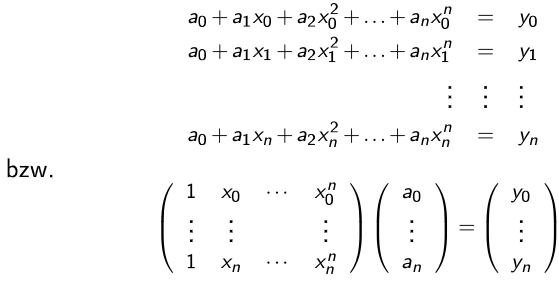
\includegraphics[scale=0.3]{interpol-poly-linearglgs}


\subsubsection{Lagrange Interpolationsformel}

Durch $n+1$ Stützpunkte mit verschiedenen Stützstellen gibt es genau EIN Polynom
$P_n(x)$ vom Grade $\le n$ welches alle Stützpunkte interpoliert.

Lagrangeform für $P_n(x)$:
$$P_n(x) = \sum_{i=0}^n l_i(x) y_i$$

Die Lagrangepolynome vom Grad $n$ ($l_i(x)$) sind definiert durch:
$$l_i(x) = \prod_{j=0, j \ne i}^n \frac{x - x_j}{x_i - x_j} \qquad \qquad i = 0,1,...,n$$

Beispiel:\\
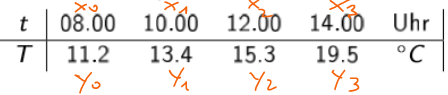
\includegraphics[scale=0.39]{interpol-poly-lagrange-bsp-data} \\
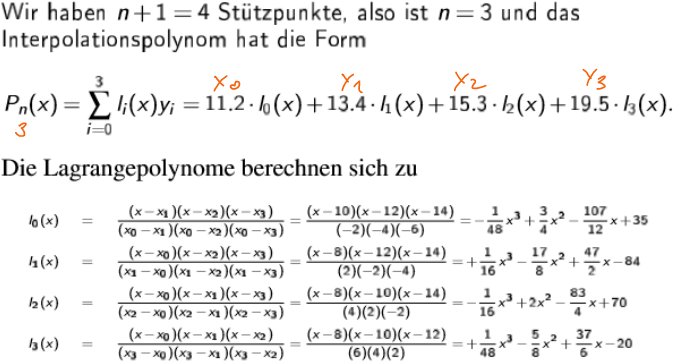
\includegraphics[scale=0.39]{interpol-poly-lagrange-bsp}


\subsubsection{Fehlerabschätzung}

Rein theoretisch weil man die tatsächliche Funktion $f$ kennen müsste.\\
Gegeben $y_i = f(x_i)$ und $f$ genügend oft stetig differenzierbar:

{
\Large
\begin{align*}
 |f(x) - P_n(x)| \quad \le \quad & \frac{|(x-x_0)(x-x_1)...(x-x_n)|}{(n+1)!}\\
                         & * \max_{x_0 \le \xi \le x_n} |f^{(n+1)}(\xi)|
\end{align*}
}



\subsection{Spline-Interpolation}

\subsubsection{Kontext}

Die Annhäherung durch ein einziges Polynom ist zwischen den Messpunkten oft
hoch instabil. Als Alternative kann stattdessen stückweise interpoliert werden.

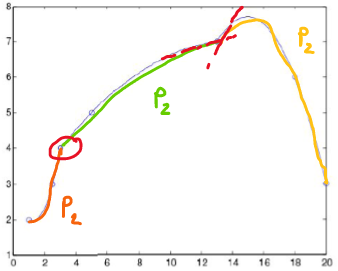
\includegraphics[scale=0.3]{interpol-split-poly-bsp}


